\documentclass{article}
\usepackage{tikz}
\usetikzlibrary{arrows.meta,decorations.pathmorphing,backgrounds,positioning,fit,petri}
\begin{document}
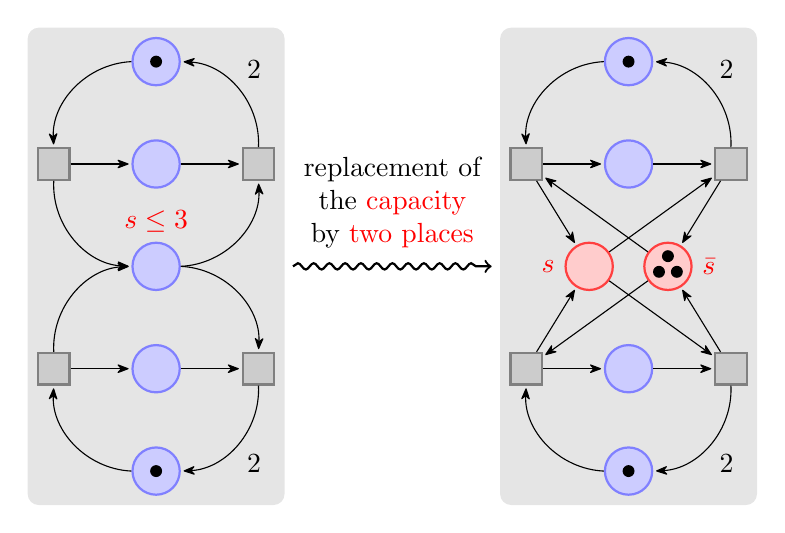
\begin{tikzpicture}[
    node distance=1.3cm,on grid,>={Stealth[round]},bend angle=45,auto,
    place/.style={circle,draw=blue!50,fill=blue!20,thick,
        inner sep=0mm,minimum size=6mm},
    transition/.style={rectangle,draw=black!50,
        fill=black!20,inner sep=0mm,minimum size=4mm,thick},
    red place/.style={place,draw=red!75,fill=red!20},
    every label/.style=red
]
 \node[place,tokens=1] (w1) {};
 \node[place] (c1) [below=of w1] {};
 \node[place] (s) [below=of c1,label=above:$s\le3$] {};
 \node[place] (c2) [below=of s] {};
 \node[place,tokens=1] (w2) [below=of c2] {};
 
 \node[transition] (e1) [left=of c1] {}
    edge[post] (c1)
    edge[pre,bend left] (w1)
    edge[post,bend right] (s);
 \node[transition] (e2) [left=of c2] {}
    edge[pre,bend right] (w2)
    edge[post, bend left] (s)
    edge[post] (c2);
 \node[transition] (l1) [right=of c1] {}
    edge[pre] (c1)
    edge[post,bend right] node[swap] {$2$} (w1)
    edge[pre,bend left] (s);
 \node[transition] (l2) [right=of c2] {}
    edge[pre] (c2)
    edge[pre,bend right] (s)
    edge[post,bend left] node {$2$} (w2);

 \begin{scope}[xshift=6cm]
 \node[place,tokens=1] (w1') {};
 \node[place] (c1') [below=of w1'] {};
 \node[red place] (s1') [below=of c1',xshift=-5mm] [label=left:$s$] {};
 \node[red place,tokens=3] (s2') [below=of c1',xshift=5mm] [label=right:$\bar s$] {};
 \node[place] (c2') [below=of s1',xshift=5mm] {};
 \node[place,tokens=1] (w2') [below=of c2'] {};
 
 \node[transition] (e1') [left=of c1'] {}
    edge[post] (c1')
    edge[pre,bend left] (w1')
    edge[post] (s1')
    edge[pre] (s2');
 \node[transition] (e2') [left=of c2'] {}
    edge[pre,bend right] (w2')
    edge[post] (s1')
    edge[pre] (s2')
    edge[post] (c2');
 \node[transition] (l1') [right=of c1'] {}
    edge[pre] (c1')
    edge[post,bend right] node[swap] {$2$} (w1')
    edge[pre] (s1')
    edge[post] (s2');
 \node[transition] (l2') [right=of c2'] {}
    edge[pre] (c2')
    edge[pre] (s1')
    edge[post] (s2')
    edge[post,bend left] node {$2$} (w2');
 \end{scope}

 \begin{scope}[on background layer]
    \node (r1) [fill=black!10,rounded corners,fit=(w1)(w2)(e1)(e2)(l1)(l2)] {};
    \node (r2) [fill=black!10,rounded corners,fit=(w1')(w2')(e1')(e2')(l1')(l2')] {};
 \end{scope}

 \draw[shorten >=1mm,-to,thick,decorate,decoration={
    snake,amplitude=.4mm,segment length=2mm,pre=moveto,
    pre length=1mm,post length=2mm
 }] (r1) -- (r2) node[above=1mm,text width=3cm,align=center,midway] {
    replacement of the \textcolor{red}{capacity}
    by \textcolor{red}{two places}
 };
\end{tikzpicture}

\end{document}

